% DGPO in piRL: 10-minute version. Build: tectonic dgpo_pirl_short.tex
% Full version with method details and backups: dgpo_pirl.tex
\documentclass[aspectratio=169,11pt]{beamer}
\usetheme{default}
\setbeamertemplate{navigation symbols}{}
\setbeamertemplate{footline}[frame number]
\setbeamerfont{frametitle}{series=\bfseries}
\definecolor{ink}{HTML}{0B0B0B}
\definecolor{ink2}{HTML}{52514E}
\definecolor{dgpo}{HTML}{2A78D6}
\definecolor{grpo}{HTML}{1BAF7A}
\setbeamercolor{frametitle}{fg=ink}
\setbeamercolor{title}{fg=ink}
\setbeamercolor{structure}{fg=dgpo}

\usepackage{booktabs}
\usepackage{graphicx}
\usepackage{tabularx}
\usepackage{array}
\graphicspath{{../figures/}}
\newcolumntype{Y}{>{\raggedright\arraybackslash}X}
\newcommand{\pirl}{$\pi$RL}
\newcommand{\pifive}{$\pi_{0.5}$}
\newcommand{\snote}[1]{{\footnotesize\textcolor{ink2}{#1}}}

\title{DGPO inside \pirl}
\subtitle{Replacing \pirl's Flow-SDE GRPO update with DGPO on \pifive}
\author{Jiyong Kwon, Purdue University}
\date{September 2026}

\begin{document}

\begin{frame}
  \titlepage
\end{frame}

\begin{frame}{Goal}
  \begin{itemize}
    \item Keep \pirl's model, simulators, rollouts and reward;
          \textbf{replace only the policy update}:
          Flow-SDE GRPO $\rightarrow$ DGPO (arXiv:2510.08425).
    \item DGPO's promise: no stochastic policy needed, so rollouts can use the
          noise-free ODE sampler; reported $\sim$20--30$\times$ faster than Flow-GRPO on images.
    \item Stage 2: replace the binary success reward with Prism's
          success $+\,\lambda\cdot$smoothness.
  \end{itemize}
\end{frame}

\begin{frame}{Experimental design}
  \footnotesize
  \begin{tabularx}{\linewidth}{@{}l Y@{}}
    \toprule
    Model & \pifive, starting from RLinf's released SFT checkpoint for each benchmark \\
    Environments & LIBERO (Spatial, Long), MetaWorld MT50, ManiSkill pick-and-place, CALVIN ABC$\rightarrow$D \\
    Methods compared & \textbf{GRPO} (\pirl, Flow-SDE noise) vs \textbf{DGPO} (ODE, or with SDE noise); optional Prism reward \\
    Same for every method & SFT start, env count, groups of 8 rollouts per reset state, 12 h on 4$\times$H100 \\
    Metric & held-out success with the \textbf{noise-free} sampler, 512 episodes per checkpoint ($\pm$2.2 pp) \\
    \bottomrule
  \end{tabularx}
  \vspace{0.5em}

  \scriptsize
  \begin{tabularx}{\linewidth}{@{}l Y Y Y Y@{}}
    \toprule
    & LIBERO & MetaWorld & ManiSkill & CALVIN \\
    \midrule
    Action & 7-d end-effector delta + gripper & 4-d xyz delta + gripper & 7-d end-effector delta + gripper & 7-d end-effector delta + gripper \\
    SFT data & 40 demos & 2,500 demos & 16,384 planner episodes & $\sim$24 h play data \\
    Reward & success 0/1 & success 0/1 & success + 0.1 grasp & subtask success \\
    SFT success (ours) & 0.806 Spatial, 0.274 Long & 0.461 & 0.447 & 0.136 \\
    \bottomrule
  \end{tabularx}
\end{frame}

\begin{frame}{The one design choice that matters: exploration noise}
  \small
  \begin{tabularx}{\linewidth}{@{}l Y Y Y@{}}
    \toprule
    & \textbf{ODE} (DGPO paper) & \textbf{SDE, every step} & \textbf{SDE, one step} (= GRPO's) \\
    \midrule
    Noise during sampling & none & 0.3 on each denoise step & 0.5 on one random step \\
    Rollout diversity & low & high & high \\
    Used by & DGPO as published & DGPO ``w/ SDE'' variant & \pirl's GRPO; DGPO control \\
    \bottomrule
  \end{tabularx}
  \vspace{0.8em}
  \begin{itemize}
    \item GRPO needs the noise (it computes the likelihood of the noised step).
    \item DGPO does not need it in principle; we test all three.
  \end{itemize}
\end{frame}

\begin{frame}{Result 1: without noise DGPO gets worse, with noise it learns}
  \centering
  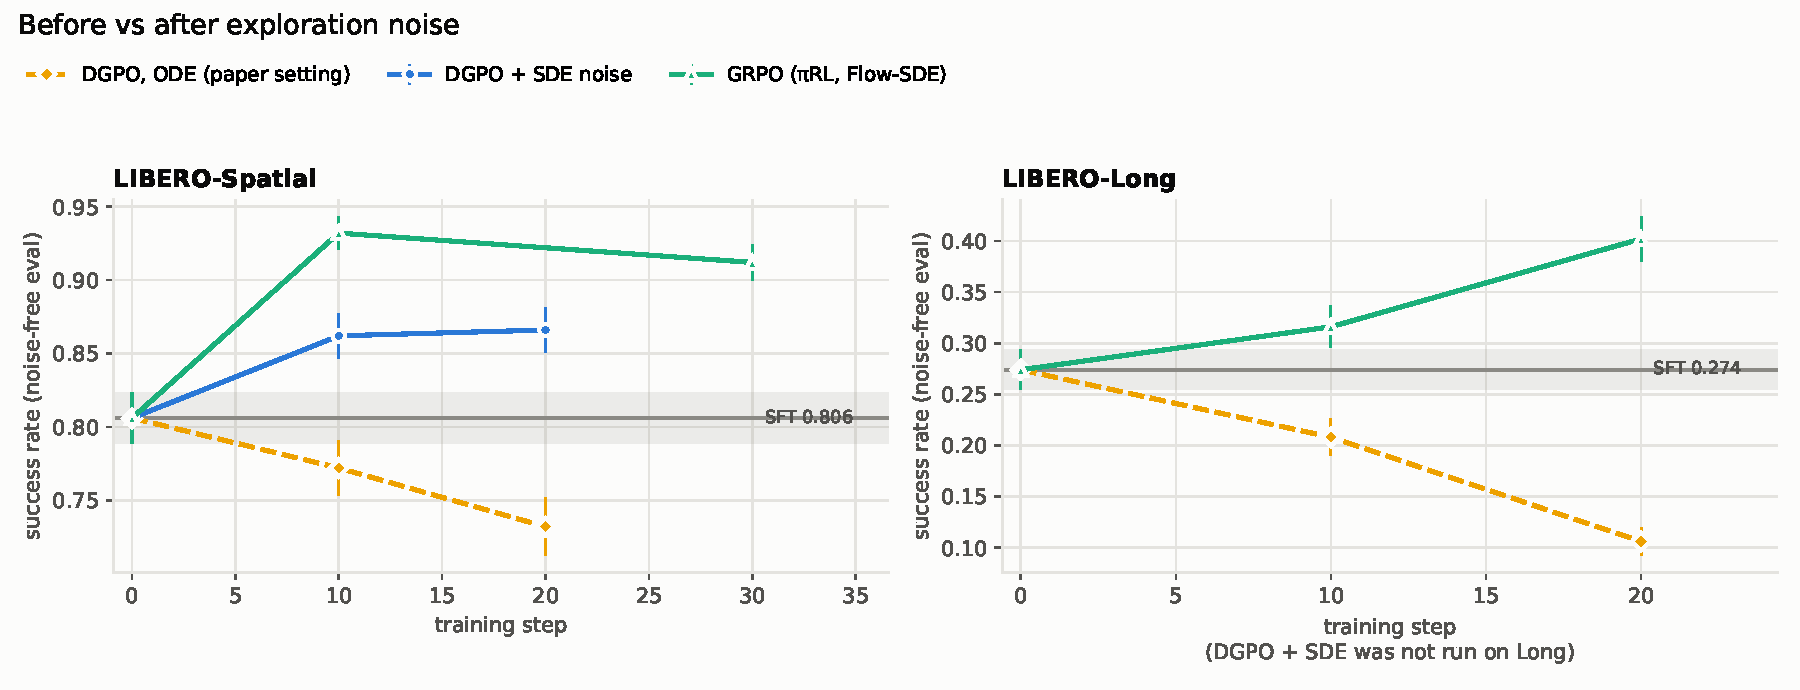
\includegraphics[width=0.95\linewidth]{fig5_noise_before_after.pdf}\\
  \snote{Grey band: SFT $\pm$1 s.e. The paper's ODE setting falls below SFT on both LIBERO suites.}
\end{frame}

\begin{frame}{Result 2: GRPO beats DGPO on every benchmark}
  \centering
  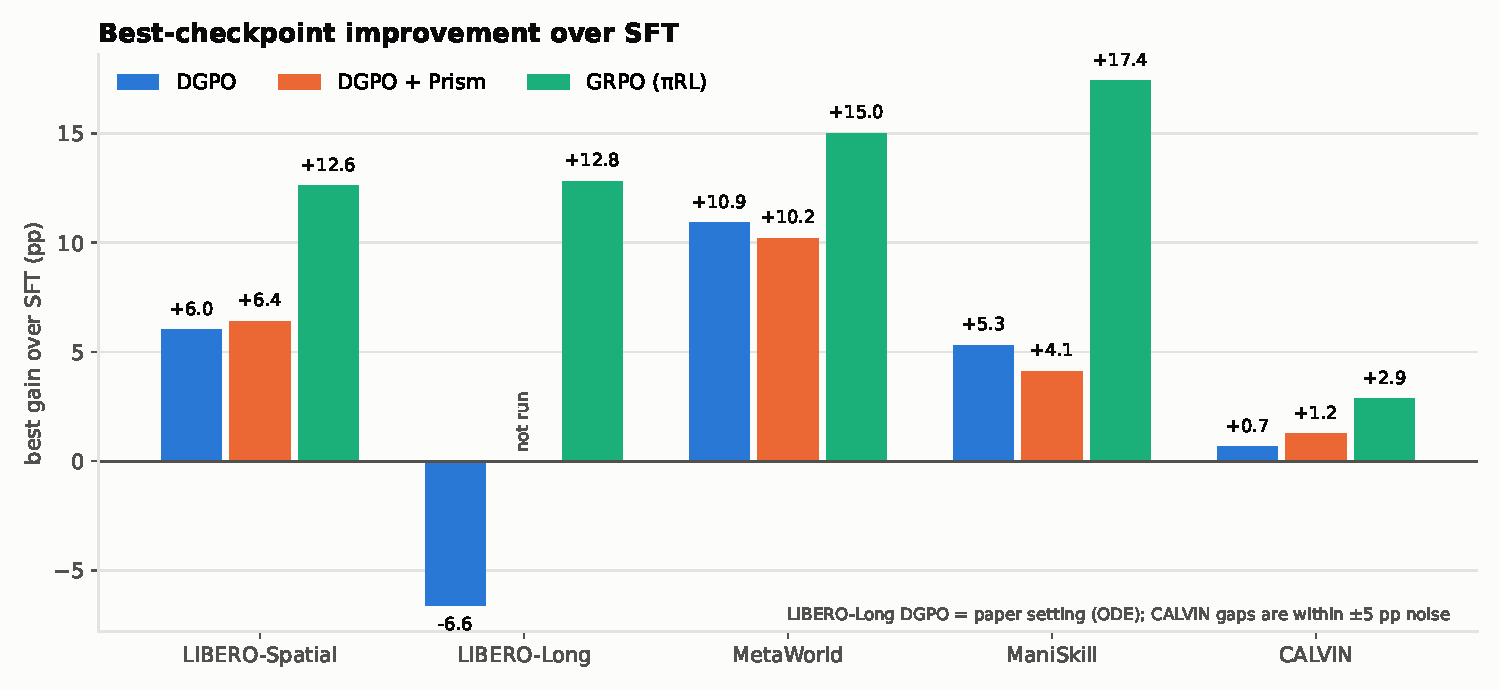
\includegraphics[width=0.9\linewidth]{fig1_summary_gain.pdf}\\
  \snote{Best checkpoint vs SFT. DGPO $=$ SDE noise on every step (LIBERO-Long: ODE only).}
\end{frame}

\begin{frame}{Result 3: learning curves}
  \centering
  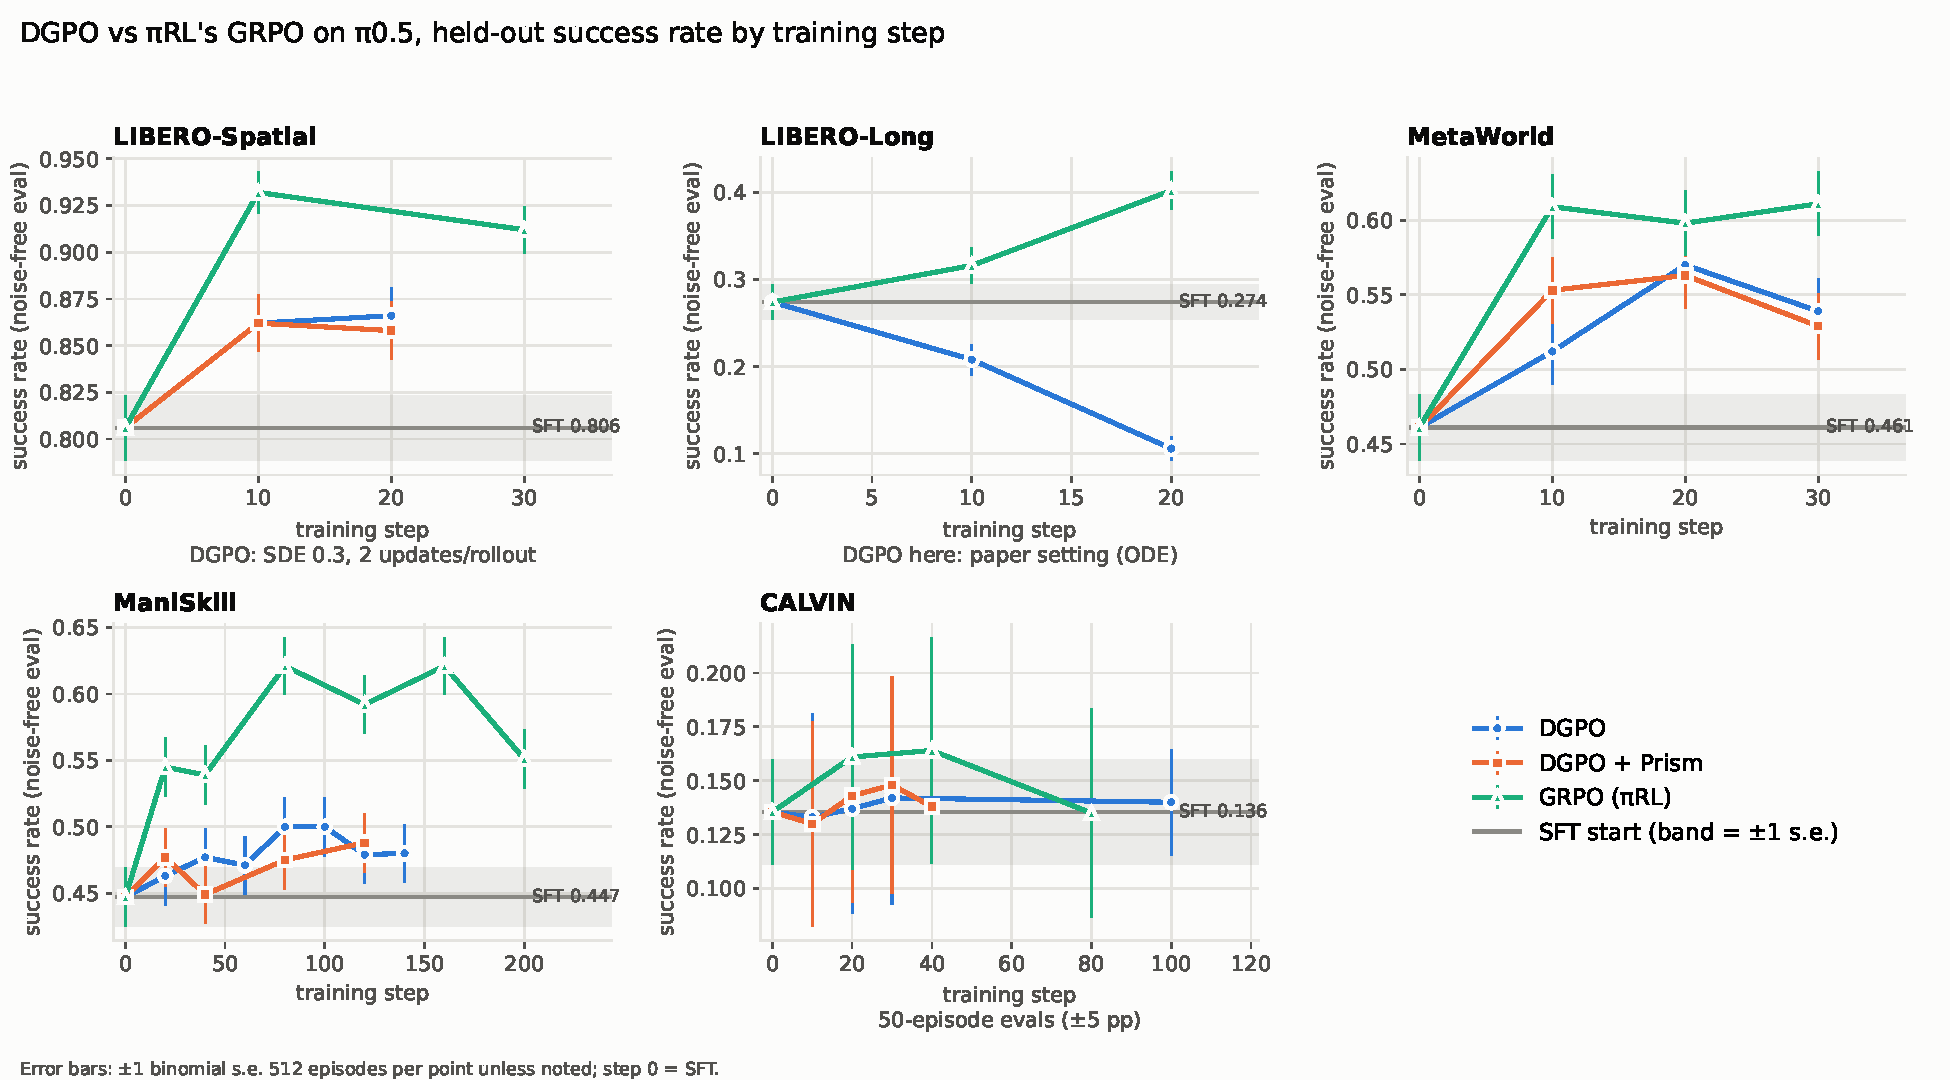
\includegraphics[width=0.93\linewidth]{fig2_learning_curves.pdf}
\end{frame}

\begin{frame}{Result 4: GRPO's exact noise does not close the gap}
  \centering
  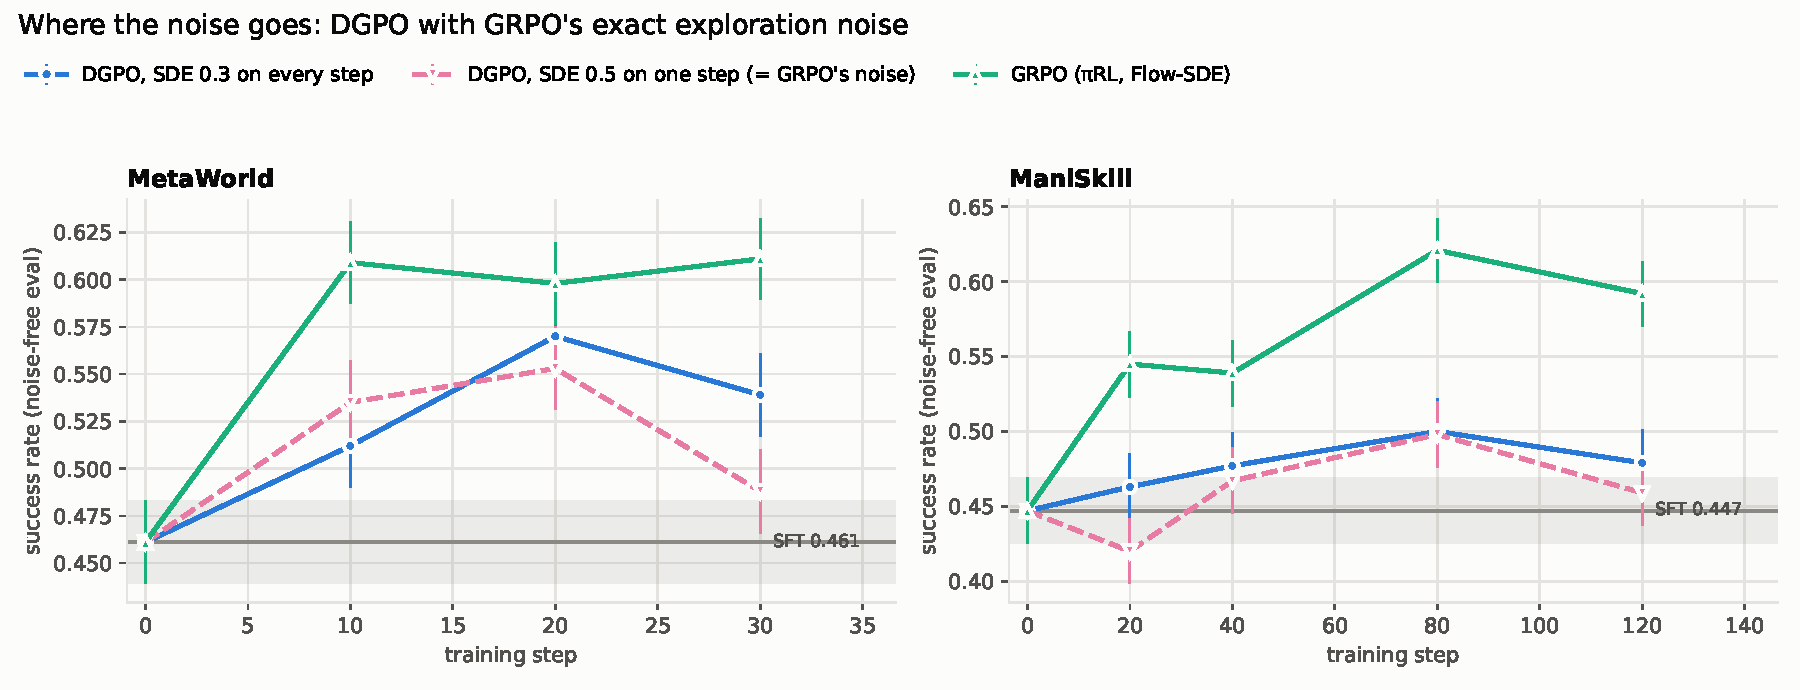
\includegraphics[width=0.95\linewidth]{fig6_noise_placement.pdf}\\
  \snote{Same rollouts as GRPO, different update only. A one-knob sweep (lr, $\beta$, updates/rollout, $t_{\min}$)
  on MetaWorld did not change this either.}
\end{frame}

\begin{frame}{Conclusions}
  \begin{itemize}
    \item \textbf{DGPO as published (ODE) makes the \pifive\ policy worse} in \pirl.
    \item With exploration noise DGPO beats SFT (LIBERO +6, MetaWorld +11, ManiSkill +5 pp),
          but \textbf{GRPO beats DGPO everywhere} (+13 / +15 / +17 pp).
    \item The gap is the update rule: our gradient matches the official DGPO code, tuning does not
          close it, and neither do identical rollouts.
    \item No speed-up: \pirl's rollouts are simulator-bound, so DGPO's savings do not apply;
          GRPO's steps were 15--35\% faster.
    \item The Prism reward adds nothing measurable; CALVIN shows no gain for any method.
  \end{itemize}
\end{frame}

\end{document}
